\documentclass[colorlinks]{thesis-kando}
\usepackage[T1]{fontenc}
\PassOptionsToPackage{defaults=hu-min}{magyar.ldf}
\usepackage[magyar]{babel}
\usepackage{graphicx,amsmath,amssymb,amsthm,hulipsum,bussproofs}
\usepackage{listings,xcolor,rotating,booktabs,fancyvrb}
\footnotestyle{rule=fourth}
\DeclareMathOperator{\tg}{tg}
\newtheorem{tetel}{Tétel}[chapter]
\usepackage[T1]{fontenc}
\PassOptionsToPackage{defaults=hu-min}{magyar.ldf}
\usepackage[magyar]{babel}
\usepackage{graphicx,amsmath,amssymb,amsthm,hulipsum,bussproofs}
\usepackage{listings,xcolor,rotating,booktabs,fancyvrb}
\footnotestyle{rule=fourth}
\newtheorem{lemma}[tetel]{Lemma}
\theoremstyle{definition}
\newtheorem{definicio}[tetel]{Definíció}
\newtheorem{feladat}[tetel]{Feladat}
\theoremstyle{remark}
\newtheorem{megjegyzes}[tetel]{Megjegyzés}
\newtheorem*{megoldas}{Megoldás}
\usepackage[utf8]{inputenc}
\usepackage[normalem]{ulem}
\usepackage{graphicx}
\usepackage{pdfpages}
\usepackage[linguistics]{forest}
\usepackage{stackengine,scalerel}

\usepackage[utf8]{inputenc} % ha még nincs
\usepackage{listings}
\usepackage{xcolor}

\lstset{
    inputencoding=utf8,
    extendedchars=true,
    literate={á}{{\'a}}1 {é}{{\'e}}1 {í}{{\'i}}1 {ó}{{\'o}}1 {ö}{{\"o}}1 {ő}{{\H{o}}}1
    {ú}{{\'u}}1 {ü}{{\"u}}1 {ű}{{\H{u}}}1
    {Á}{{\'A}}1 {É}{{\'E}}1 {Í}{{\'I}}1 {Ó}{{\'O}}1 {Ö}{{\"O}}1 {Ő}{{\H{O}}}1
    {Ú}{{\'U}}1 {Ü}{{\"U}}1 {Ű}{{\H{U}}}1,
    breaklines=true,
    basicstyle=\ttfamily\small,
    keywordstyle=\color{blue},
    commentstyle=\color{gray},
    stringstyle=\color{teal}
}


% Define JavaScript language for listings
\lstdefinelanguage{JavaScript}{
    keywords={break, case, catch, continue, debugger, default, delete, do, else, finally, for, function, if, in, instanceof, new, return, switch, this, throw, try, typeof, var, void, while, with, let, const, export, import, await, async},
    ndkeywords={class, export, boolean, throw, implements, import, this, new},
    sensitive=true,
    comment=[l]{//},
    morecomment=[s]{/*}{*/},
    morestring=[b]',
    morestring=[b]",
    alsoletter={-},
    alsodigit={:},
    morekeywords=[2]{=>, yield, async, await, constructor},
    keywordstyle=\color{blue}\bfseries,
    ndkeywordstyle=\color{green}\bfseries,
    identifierstyle=\color{black},
    commentstyle=\color{gray}\ttfamily,
    stringstyle=\color{red}\ttfamily,
}

% Customize listings appearance
\lstset{
    language=JavaScript,
    extendedchars=true,
    inputencoding=utf8,
    basicstyle=\ttfamily\small,
    numbers=left,
    numberstyle=\tiny\color{gray},
    stepnumber=1,
    numbersep=10pt,
    showstringspaces=false,
    breaklines=true,
    frame=single,
    captionpos=b,
    escapeinside={\%*}{*)},
}

% Fordított 'T' szimbólum definiálása
\def\tang{\ThisStyle{\abovebaseline[0pt]{\scalebox{-1}{$\SavedStyle\perp$}}}}

\begin{document}


\title{Project Hephaistos}

\author{Biliczki Bence\\Fodor Valentin Sándor\\Szegedi Dávid\\Szoftverfejlesztő és -tesztelő szak}

\supervisor{Kerényi Róbert Nándor\\oktató}
\city{Miskolc}
\date{2024}
\begin{figure}[h]
    \centering
    \label{fig:minta}
\end{figure}
\maketitle

\tableofcontents

\pagebreak

\section*{Bevezetés} \addcontentsline{toc}{section}{Bevezetés}

A Project Hephaistos egy innovatív, egyetemisták számára készült órarend-tervező alkalmazás, amely célja, hogy hatékonyan támogassa a hallgatókat az órák, tanórán kívüli tevékenységek és egyéb kötelezettségek rendszerezésében. Az alkalmazás CS nyelven készült, és egy gépészmérnökhallgató igényei alapján lett fejlesztve, különös figyelmet szentelve a funkcionalitásnak és a felhasználóbarát felületnek. Az intelligens ütemezési megoldások lehetővé teszik az egyéni preferenciák, az egyetemi órarend és az időbeli ütközések figyelembevételét.

\section{Használt Technológiák}
A Hephaistos projekt különböző, modern technológiákat alkalmaz a backend, frontend fejlesztéséhez, valamint az adatbázis kezeléséhez. A backend fejlesztés során erőteljes és skálázható megoldásokat biztosítanak, például Node.js használatával, amelyek lehetővé teszik a gyors, aszinkron feldolgozást és az API-k kialakítását. A backend kezelheti a felhasználói adatokat, autentikációt, valamint biztosítja az alkalmazás logikai rétegeit, és kezeli a kommunikációt az adatbázissal.

A frontend fejlesztésére a projekt React környezetben dolgozik, hogy dinamikus, interaktív felhasználói felületeket kínáljon, amelyek gyorsan reagálnak a felhasználói interakciókra. Ezek a könyvtárak lehetővé teszik a komponens-alapú struktúrák kialakítását, így a fejlesztés hatékonyabb és karbantarthatóbb lesz. A CSS preprocesorok és UI frameworkök (pl. Material-UI, Bootstrap) tovább javítják a felhasználói élményt és az alkalmazás megjelenését.

Az adatbázis-kezeléshez a projekt fejlesztése során MySQL relációs adatbázist használunk, amely lehetővé teszi az adatok hatékony tárolását és gyors lekérdezését. A backend és az adatbázis közötti kommunikációt közvetlen SQL lekérdezések segítségével végezzük, amelyek egyszerűsítik az adatok kezelését és lekérdezését az alkalmazás logikai rétegében. A projekt publikálása után az adatbázis az Azure felhőszolgáltatáson keresztül kerül elérhetővé, biztosítva a skálázhatóságot, megbízhatóságot és biztonságot a termelési környezetben. A Hephaistos projekt által használt technológiai stack elősegíti a rugalmas, skálázható és könnyen karbantartható alkalmazások fejlesztését, biztosítva a zökkenőmentes integrációt a backend, frontend és az adatbázis között.

\subsection{Backend}
A projekt backend fejlesztéséhez a .NET Core keretrendszert használjuk, amely egy nyílt forráskódú, platformfüggetlen fejlesztői környezet. A .NET Core lehetővé teszi a fejlesztők számára, hogy modern, felhőalapú alkalmazásokat építsenek, amelyek nagy teljesítményűek és könnyen skálázhatók. A keretrendszer előnye, hogy több operációs rendszeren is működik, beleértve a Windows, Linux és macOS platformokat, így rugalmas fejlesztési lehetőségeket kínál A .NET Core különösen jól támogatja a mikroszolgáltatás-alapú architektúrákat, így lehetőség van az alkalmazás kisebb, jól elkülöníthető szolgáltatásokra bontására. Ez nemcsak a karbantarthatóságot növeli, hanem biztosítja a magas rendelkezésre állást és skálázhatóságot is. Az integrációs lehetőségek, például a Microsoft Azure-val való zökkenőmentes együttműködés, lehetővé teszik a felhőszolgáltatások egyszerű használatát. A fejlesztés során az Entity Framework Core biztosítja az adatok kezelését, egyszerűsítve az adatbázisokkal való munkát, miközben a web API-k gyors létrehozására is lehetőséget ad, támogatva a RESTful szolgáltatásokat. Ezzel biztosítva van a könnyű adatkommunikáció a frontend és backend között.

\subsubsection{ASP.NET Core}
Az ASP.NET Core a .NET Core keretrendszer része, amelyet webalkalmazások és API-k fejlesztésére használnak. Az ASP.NET Core előnyei közé tartozik a magas teljesítmény, a platformfüggetlenség és a moduláris felépítés. Az ASP.NET Core támogatja a modern webfejlesztési szabványokat és eszközöket, mint például a dependency injection, a middleware-ek és a RESTful API-k.

Az ASP.NET Core alkalmazások könnyen telepíthetők és skálázhatók, így ideálisak a felhőalapú környezetekben történő futtatásra. Az ASP.NET Core lehetővé teszi a fejlesztők számára, hogy gyorsan és hatékonyan hozzanak létre biztonságos és megbízható webalkalmazásokat.

\subsection{Adatbázis}
Az adatok tárolására MySQL adatbázist használunk. A MySQL egy népszerű, nyílt forráskódú relációs adatbázis-kezelő rendszer, amely nagy teljesítményt és megbízhatóságot kínál. A PHPMyAdmin eszközt használjuk az adatbázis kezelésére, amely egy webalapú felületet biztosít az adatbázisok kezeléséhez.

\subsection{Frontend}
A React egy népszerű JavaScript-könyvtár, amelyet dinamikus és interaktív felhasználói felületek (UI) fejlesztésére használnak. A React lehetővé teszi a fejlesztők számára, hogy komponens-alapú módon építsenek fel alkalmazásokat, ahol minden komponens saját állapotot és viselkedést tartalmaz. A virtuális DOM használata gyorsabb renderelést biztosít, mivel csökkenti a tényleges DOM-műveletek számát. A React alkalmazásokat könnyen skálázhatjuk és karbantarthatjuk, és a könyvtár számos kiegészítő eszközt kínál, mint például Redux az állapotkezeléshez, vagy React Router a navigációhoz. Emellett a React lehetőséget ad mobilalkalmazások készítésére is React Native segítségével.



\subsubsection{React}
A React egy komponens-alapú JavaScript könyvtár, amelyet a Meta fejlesztett ki és 2013-ban adtak ki. A React fő célja a felhasználói felületek egyszerűbb és hatékonyabb fejlesztése. A React lehetővé teszi a fejlesztők számára, hogy újrafelhasználható komponenseket hozzanak létre, amelyek könnyen karbantarthatók és bővíthetők.

A React egyik legfontosabb jellemzője a virtuális DOM (Document Object Model), amely javítja az alkalmazás teljesítményét azáltal, hogy minimalizálja a valódi DOM manipulációkat. A React támogatja a JSX (JavaScript XML) szintaxist, amely lehetővé teszi a HTML-szerű kód írását a JavaScript-ben, növelve a kód olvashatóságát és karbantarthatóságát.

A React ökoszisztémája számos kiegészítő könyvtárat és eszközt tartalmaz, mint például a React Router a kliensoldali útvonalkezeléshez és a Redux az állapotkezeléshez. Ezek az eszközök segítenek a fejlesztőknek hatékonyabb és skálázhatóbb alkalmazásokat létrehozni.

\subsection{Fejlesztői Eszközök}
A fejlesztés során különböző eszközöket használunk a hatékonyság növelése és a hibakeresés megkönnyítése érdekében:
\begin{itemize}
    \item \textbf{Visual Studio Code (VSCode)}: Egy népszerű kódszerkesztő, amely számos bővítménnyel rendelkezik, például az \texttt{ESLint} és \texttt{Prettier} segítségével.
    \item \textbf{React Developer Tools}: Egy böngészőbővítmény, amely lehetővé teszi a React komponensek és állapotok ellenőrzését a böngészőben.
    \item \textbf{PHPMyAdmin}: Egy webalapú eszköz a MySQL adatbázisok kezelésére.
\end{itemize}

\section{Projekt Felépítése}
A Hephaistos projekt három fő komponensből áll: backend, frontend és adatbázis. Az alábbiakban bemutatjuk ezeknek a komponenseknek a felépítését és funkcióit.

\section{Órarend Generátor Funkció}
A Project Hephaistos backend tartalmaz egy órarend generátor funkciót, amely segíti a felhasználókat az optimális órarend összeállításában. Ez a funkció figyelembe veszi a felhasználó által teljesített tantárgyakat, a tantárgyak előfeltételeit, valamint az időbeli ütközéseket.

\subsection{TimetableGenerator Osztály}
A \texttt{TimetableGenerator} osztály felelős az órarend generálásáért. Az osztály a következő fő metódust tartalmazza:

\begin{itemize}
    \item \textbf{GenerateClosestTimetable}: Ez a metódus a megadott kreditszám alapján generál egy optimális órarendet. A metódus figyelembe veszi az elérhető tantárgyakat és az ütemezési konfliktusokat.
\end{itemize}

Az alábbi kód egy részletet mutat be a \texttt{GenerateClosestTimetable} metódusból:

\begin{lstlisting}[language=JavaScript]
public (IEnumerable<SubjectSchedule> Timetable, IEnumerable<Subject> OmittedSubjects) GenerateClosestTimetable(
    int creditValue,
    List<Subject> _availableSubjects,
    List<SubjectSchedule> _existingSchedules
) {
    var selectedSubjects = new List<Subject>();
    var omittedSubjects = new List<Subject>();
    var selectedSchedules = new List<SubjectSchedule>();
    int totalCredits = 0;

    foreach (var subject in _availableSubjects) {
        if (totalCredits + (subject.CreditValue ?? 0) > creditValue) {
            omittedSubjects.Add(subject);
            continue;
        }

        var subjectSchedules = _existingSchedules.Where(s => s.SubjectId == subject.Id).ToList();

        if (!subjectSchedules.Any(schedule => IsOverlapping(schedule, selectedSchedules))) {
            selectedSubjects.Add(subject);
            selectedSchedules.AddRange(subjectSchedules);
            totalCredits += subject.CreditValue ?? 0;
        } else {
            omittedSubjects.Add(subject);
        }
    }

    return (selectedSchedules, omittedSubjects);
}
\end{lstlisting}

\subsection{TimetableGeneratorController Végpont}
A \texttt{TimetableGeneratorController} egy API végpontot biztosít az órarend generálásához. A végpont a következőképpen működik:

\begin{itemize}
    \item \textbf{POST /api/timetablegenerator/generate}: Ez a végpont fogadja a felhasználó által megadott kreditszámot, és visszaadja az optimális órarendet, valamint azokat a tantárgyakat, amelyek kimaradtak az ütemezésből.
\end{itemize}

Az alábbi kód egy részletet mutat be a végpont implementációjából:

\begin{lstlisting}[language=JavaScript]
[HttpPost("generate")]
[Authorize]
public async Task<IActionResult> GenerateTimetable([FromBody] int creditValue, [FromHeader(Name = "Authorization")] string Authorization) {
    var userId = _jwtHelper.ExtractUserIdFromToken(Authorization);
    var availableSubjects = GetAvailableSubjects(userId.Value);
    var existingSchedules = _context.Subjectschedules
        .Where(schedule => availableSubjects.Any(subject => subject.Id == schedule.SubjectId))
        .ToList();

    var (timetable, omittedSubjects) = _timetableGenerator.GenerateClosestTimetable(creditValue, availableSubjects, existingSchedules);

    return Ok(new {
        Timetable = timetable.Select(schedule => new {
            SubjectName = schedule.Subject?.Name,
            DayOfWeek = schedule.DayOfWeek,
            StartTime = schedule.StartTime,
            EndTime = schedule.EndTime
        }),
        OmittedSubjects = omittedSubjects.Select(subject => new {
            SubjectName = subject.Name
        })
    });
}
\end{lstlisting}

\subsection{Felhasználói Élmény}
A funkció biztosítja, hogy a felhasználók egy könnyen értelmezhető és áttekinthető órarendet kapjanak, amely tartalmazza az órák nevét, időpontját és napját, így a tanulók gyorsan ráláthatnak napi és heti beosztásukra. Az órarend minden órát megfelelő időpontban és napra rendezve jelenít meg, figyelembe véve a tantárgyak közötti ütközéseket és azok optimális elosztását. A felhasználói élmény javítása érdekében az órarend könnyen navigálható, és biztosítja, hogy a tanulók minden szükséges információt megtaláljanak. Amennyiben egy tantárgy valamilyen okból nem került be az órarendbe, a rendszer egy külön listában jeleníti meg azokat az órákat, amelyek kimaradtak, lehetővé téve a felhasználók számára, hogy tisztában legyenek azzal, mely tantárgyak nem szerepelnek az ütemezésben. Ez segít elkerülni az esetleges hiányosságokat, és biztosítja, hogy a tanulók tisztában legyenek azokkal a tantárgyakkal, amelyeket még nem tudtak beilleszteni. Továbbá, a rendszer lehetőséget ad arra, hogy a felhasználók az egyes órákra kattintva részletes információkat is elérhessenek, például az oktató nevét, az órák helyszínét és esetleges házi feladatokat vagy egyéb fontos tudnivalókat. A kimaradó tantárgyak esetében a felhasználók szűrőfunkciókat is alkalmazhatnak, így könnyen kereshetnek a listában, és információkat kaphatnak arról, hogy miért nem szerepel az adott tantárgy az órarendjükben, vagy milyen alternatív megoldások léteznek annak beillesztésére.

\chapter{Relációs adatkezelő rendszerek}

\section{Relációs adatbázis}

Relációs adatbázisnak nevezzük azokat az adatbázisokat, amelyek a relációs adatmodell elvein alapulnak. Ezekben az adatok táblázatos formában, ún. relációkban (táblákban) vannak tárolva, ahol a sorok egyedi rekordokat, az oszlopok pedig mezőket (attribútumokat) jelentenek. A relációs adatbázis több ilyen táblát tartalmaz, amelyeket egymással kapcsolatokon (kulcsokon) keresztül lehet összekötni. Az ilyen adatbázisokat relációs adatbázis-kezelő rendszerek (pl. MySQL, PostgreSQL, SQL Server) segítségével lehet létrehozni, módosítani és kezelni. Az adatok lekérdezésére és módosítására jellemzően az SQL nyelvet használjuk. A relációs adatbázisok erőssége a strukturált adattárolás, a konzisztencia és az adatintegritás biztosítása.

\subsection{A relációs adatbáziskezelő rendszerek}

A relációs adatbáziskezelő rendszerek (RDBMS, azaz Relational Database Management System) olyan szoftverek, amelyek az adatokat táblák formájában kezelik. Minden tábla oszlopokból és sorokból áll, ahol az oszlopok különböző attribútumokat jelölnek, míg a sorok egyedi rekordokat reprezentálnak. Az RDBMS-ekben a táblák között relációk, azaz kapcsolatok hozhatók létre, így biztosítva az adatok egymáshoz kapcsolódó kezelését.

Az RDBMS-ek egyik legfontosabb jellemzője a strukturált lekérdezőnyelv, azaz az SQL (Structured Query Language), amely lehetővé teszi az adatok lekérdezését, módosítását és kezelését. Az adatokat kulcsok segítségével kapcsoljuk össze, mint például az elsődleges kulcs (primary key) és az idegen kulcs (foreign key). Az adatok normalizálásával csökkenthetők az ismétlődések, és fenntartható az adatintegritás. A relációs adatbáziskezelő rendszerek széles körben elterjedtek különböző üzleti és technológiai területeken, mivel lehetővé teszik az adatok hatékony tárolását és kezelését, valamint a nagy mennyiségű adat gyors lekérdezését.
\pagebreak
\subsection{MySQL és MariaDB, valamint PHPMyAdmin}

A MySQL és a MariaDB két népszerű, nyílt forráskódú relációs adatbáziskezelő rendszer. Mindkettő hasonló struktúrát és működési elveket követ, mivel a MariaDB a MySQL-ből származik. A MySQL-t eredetileg a Sun Microsystems fejlesztette ki, majd a Sun felvásárlása után az Oracle tulajdonába került. A MariaDB-t a MySQL eredeti fejlesztői hozták létre az Oracle irányításától való függetlenség megőrzése érdekében, és azóta külön fejlesztési irányt követ.

Mindkét rendszer könnyen kezelhető, nagy teljesítményt és skálázhatóságot kínál, így gyakran használják webalkalmazások és más dinamikus rendszerek adatbázisaként. A MySQL és a MariaDB támogatják a különféle táblastruktúrákat (például InnoDB és MyISAM), a tranzakciókezelést, valamint a különféle biztonsági mechanizmusokat, mint például a felhasználói jogosultságok finomhangolása.

A PHPMyAdmin egy népszerű, nyílt forráskódú webes eszköz, amelyet kifejezetten MySQL és MariaDB adatbázisok kezelésére fejlesztettek ki. Lehetővé teszi a felhasználók számára, hogy grafikus felületen keresztül, SQL parancsok írása nélkül menedzseljék az adatbázisokat. Ezzel az eszközzel könnyen létrehozhatók és módosíthatók táblák, kezelhetők a felhasználói jogosultságok, és futtathatók különböző SQL lekérdezések.

A PHPMyAdmin előnye, hogy böngésző alapú, így bármilyen eszközről könnyen elérhető, nem szükséges hozzá parancssori ismeret. A felhasználók könnyen átláthatják az adatbázis struktúráját, létrehozhatnak exportálási és importálási műveleteket, valamint automatikusan generált diagramok segítségével áttekinthetik a táblák közötti kapcsolatokat. Ezen kívül a PHPMyAdmin lehetőséget biztosít biztonsági mentések készítésére, így a felhasználók megőrizhetik és helyreállíthatják az adatokat.

\begin{figure}[ht!]
    \centering
    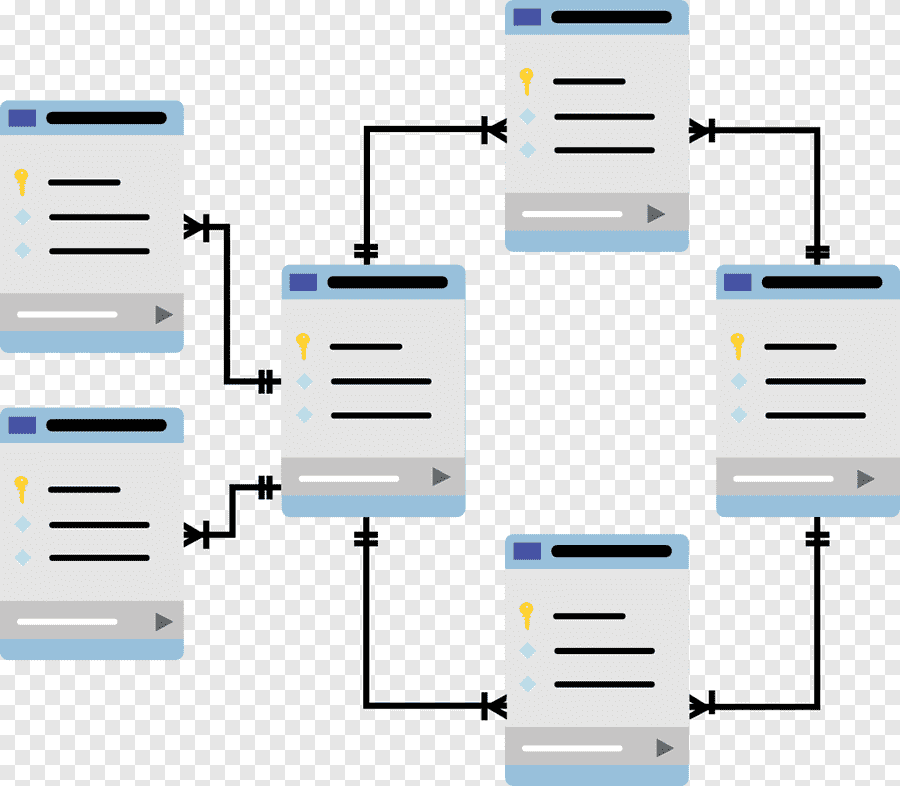
\includegraphics[width=9cm]{figures/rdb.png}
    \caption[dotNET]{Relációs adatbázis}
\end{figure}
\pagebreak

\chapter{React Fejlesztői Környezet}

\section{Bevezetés}
A React egy népszerű JavaScript-könyvtár, amelyet a felhasználói felületek egyszerűbb fejlesztésére használnak. Ezt a Meta fejlesztette, és 2013-ban adták ki. Azóta széles körben alkalmazzák a webes fejlesztésben, különösen az egyoldalas alkalmazások (SPA) készítéséhez. Ez a szakdolgozat a React fejlesztői környezetek felépítését, a szükséges eszközöket és a hatékony fejlesztéshez szükséges alapelveket vizsgálja.

\section{React Fejlesztői Környezet}
A React fejlesztői környezet beállítása az első lépés a sikeres alkalmazásfejlesztéshez. Ehhez szükséges a Node.js és az npm telepítése, amelyek biztosítják a JavaScript futtatókörnyezetet és a csomagkezelést. A React alkalmazások gyors indításához a create-react-app eszköz használata javasolt, amely előre konfigurált fejlesztési környezetet biztosít. A React alapja a komponens-alapú felépítés, amely lehetővé teszi az alkalmazások moduláris felépítését és könnyebb karbantartását. A JSX szintaxis segítségével a JavaScript és HTML kód egyszerűen kombinálható, növelve a kód olvashatóságát. A state és props kezelésével pedig dinamikusan irányíthatjuk az alkalmazás adatfolyamát és a felhasználói interakciókat. A megfelelő környezet beállításával és az alapok elsajátításával gyorsan elérhetjük a React alkalmazás fejlesztésének sikeres elindítását.

\subsection{React Telepítése és Projektindítás}
A React telepítéséhez először szükségünk van a Node.js és npm (Node Package Manager) telepítésére, amelyek segítségével kezelhetjük a JavaScript könyvtárakat és függőségeket. Miután a Node.js és az npm telepítve van, létrehozhatunk egy új React projektet az \texttt{create-react-app} eszközzel.

Az alábbi parancsokkal létrehozható egy új React projekt:
\begin{lstlisting}[language=bash]
npx create-react-app my-app
cd my-app
npm start
\end{lstlisting}

\pagebreak

A \texttt{create-react-app} gyorsan felállít egy alap React projektstruktúrát, amely a következő fájlokat tartalmazza:
\begin{itemize}
    \item \texttt{src/} mappa: a projekt alapvető forráskódját tartalmazza, és ebben található minden olyan fájl, amely az alkalmazás működéséhez szükséges. A mappa tartalmazza a komponensek fájljait, amelyek a felhasználói felület különböző részeit alkotják, valamint az alkalmazás logikáját, amely kezeli a különböző funkcionalitásokat, adatkezelést és interakciókat. A komponensek hierarchikus felépítésében a fejlesztők könnyen megtalálják a különböző funkciókhoz tartozó részeket, ezáltal segítve a karbantartást és a bővítést.
    \item \texttt{public/} mappa: a projekt statikus fájljait tartalmazza, amelyek közvetlenül elérhetők a böngészőből, és nem igényelnek semmilyen feldolgozást a build folyamat során. Ide tartoznak a különböző statikus fájlok, mint például képek, ikonszettek, betűtípusok és más, az alkalmazásban használt fix fájlok, amelyek nem változnak az alkalmazás működése közben.
    \item \texttt{node\_modules/}: tartalmazza az alkalmazás számára szükséges összes külső függőséget és csomagot, amelyeket a projekt telepítése során a npm (Node Package Manager) segítségével töltünk le. Ebbe a mappába kerülnek az összes könyvtár és csomag, amelyeket a projekt kódja futtatásához szükséges, például React, utility könyvtárak, tesztelési keretrendszerek, és egyéb fejlesztői eszközök.
\end{itemize}

\subsection{Fejlesztői Eszközök}
A React fejlesztéséhez számos fejlesztői eszköz áll rendelkezésünkre, amelyek növelhetik a termelékenységet és a hibakeresés hatékonyságát.


\subsubsection{React Developer Tools}
A React Developer Tools egy hivatalos böngészőbővítmény, amely lehetővé teszi a React alapú webalkalmazások mélyreható vizsgálatát és hibakeresését közvetlenül a böngésző fejlesztői eszközein belül. A bővítmény segítségével a fejlesztők átlátható módon megtekinthetik az alkalmazás teljes komponensfáját, beleértve a komponensek közötti hierarchiát és kapcsolatokat. Különösen hasznos funkciója, hogy lehetővé teszi az egyes komponensekhez tartozó props és state értékek valós idejű megfigyelését, illetve ezek változásainak nyomon követését a felhasználói interakciók során. A modern React fejlesztés során gyakran használt Hook-ok – mint például a useState, useEffect, vagy useContext – szintén jól követhetők a bővítményen keresztül, így a fejlesztők részletes információt kaphatnak az alkalmazás belső állapotairól. Ezen kívül a React Developer Tools egy beépített profilozó eszközt is tartalmaz, amely lehetővé teszi a komponensrenderelések teljesítményének elemzését, megmutatva, hogy mely komponensek renderelődnek újra, milyen gyakorisággal, és mennyi idő alatt. Mindezek együttesen nagyban hozzájárulnak a hatékonyabb hibakereséshez, az optimalizáláshoz, és az alkalmazás működésének jobb megértéséhez, ezáltal elengedhetetlenné téve a bővítményt minden komolyabb React fejlesztési projekt során.

\section{React Alapjai}
A React egy összetevő-alapú megközelítést alkalmaz, amely lehetővé teszi, hogy az alkalmazás kisebb, újrafelhasználható komponensekből épüljön fel. Mivel minden komponens saját állapotot és viselkedést kezelhet, az alkalmazás könnyen kezelhető és bővíthető. Ez a moduláris felépítés elősegíti a kód karbantartását, mivel a különböző komponensek függetlenül fejleszthetők, tesztelhetők és frissíthetők anélkül, hogy az alkalmazás többi része károsodna. A komponens-alapú struktúra lehetővé teszi a kód logikai szétválasztását és az újrafelhasználhatóságot. Egy-egy komponens akár több helyen is alkalmazható, így a fejlesztők elkerülhetik az ismétlődő kódok írását, ami növeli a fejlesztés hatékonyságát. Emellett a komponensek izoláltsága segíti a hibakeresést, mivel könnyen beazonosítható, hogy melyik rész felelős egy adott viselkedésért vagy hibáért. Ez a megközelítés nemcsak a fejlesztés gyorsításában, hanem a csapatmunkában is előnyt jelent, mivel a különböző fejlesztők párhuzamosan dolgozhatnak a különböző komponenseken. A React ezáltal biztosítja, hogy az alkalmazás nagy méretű és összetett funkciók mellett is skálázható és rugalmas maradjon, miközben a kód alapja átlátható és jól struktúrált.

Ez a változat hangsúlyozza a moduláris felépítést, az újrafelhasználhatóságot és a karbantarthatóságot, és azt, hogy ezek hogyan segítik a gyorsabb fejlesztést és a jobb csapatmunkát. Ha bármit szeretnél finomítani, csak szólj!

\subsection{Komponensek és JSX}
A React komponensek JavaScript függvények vagy osztályok, amelyek HTML-szerű kódot, úgynevezett JSX-et használnak. A JSX egy szintaxisbővítés, amely lehetővé teszi, hogy a JavaScript kódban HTML elemeket írjunk, miközben megőrizzük a JavaScript teljes funkcionalitását. A JSX segít abban, hogy a kód olvashatóbbá váljon, mivel a logikai struktúrák és a megjelenítés közvetlenül egymás mellett találhatóak. A JSX-ben írt HTML szerű kód valójában nem közvetlenül HTML, hanem JavaScript kifejezésekké fordul le, amit a React futtatáskor képes renderelni. Ez lehetővé teszi a dinamikus tartalom generálását, mivel a komponens kódjában szereplő adatokat vagy logikai feltételeket is könnyen integrálhatjuk a megjelenítésbe. A JSX alapvetően javítja a kód karbantartását és bővíthetőségét, mivel az alkalmazás minden része (adatok, logika és megjelenítés) egy helyen, tiszta és érthető módon van strukturálva. A JSX nemcsak a statikus HTML elemeket támogatja, hanem lehetőséget ad arra is, hogy JavaScript kifejezéseket ágyazzunk be, mint például változókat, függvényhívásokat vagy ciklusokat. Mivel végül a JSX JavaScript-re fordítódik, így a böngésző számára is érthető és végrehajtható kódot eredményez, miközben megőrzi a dinamikus viselkedést és a felhasználói interakciók kezelését. A React alkalmazásokban a JSX alapú komponensek lehetővé teszik a újrafelhasználható kódok létrehozását, így a fejlesztők gyorsan és hatékonyan tudják kezelni az alkalmazás felhasználói felületét. A JSX és a React együtt biztosítják, hogy az alkalmazás rugalmasan alkalmazkodjon a különböző felhasználói igényekhez, miközben könnyen bővíthető és karbantartható marad.

\section*{Microsoft Azure Elérhetőség}
\addcontentsline{toc}{section}{Microsoft Azure Elérhetőség}
A Project Hephaistos alkalmazásunkat a Microsoft Azure felhőszolgáltatás segítségével publikáltuk, amely lehetővé teszi a skálázható és megbízható működést. Az Azure biztosítja az alkalmazás számára a szükséges infrastruktúrát, beleértve a webalkalmazás hosztolását, az adatbázis-kezelést és a biztonságos hozzáférést.

Az alkalmazás elérhető az alábbi linken:
\url{https://hephaistos-backend-c6c5ewhraedvgzex.germanywestcentral-01.azurewebsites.net/index.html}

\subsection*{Azure Szolgáltatások Használata}
A projekt során az alábbi Azure szolgáltatásokat használtuk:
\begin{itemize}
    \item \textbf{Azure App Service}: Az alkalmazás hosztolására és futtatására használtuk. Ez egy teljesen menedzselt platform, amely lehetővé teszi a gyors telepítést és a folyamatos integrációt.
    \item \textbf{Azure SQL Database}: Az alkalmazás adatainak tárolására és kezelésére szolgál. Ez egy skálázható, biztonságos és megbízható relációs adatbázis-kezelő rendszer.
    \item \textbf{Azure Monitor}: Az alkalmazás teljesítményének és állapotának nyomon követésére használtuk. Ez segít az esetleges problémák gyors azonosításában és megoldásában.
    \item \textbf{Azure Active Directory (AAD)}: A felhasználók hitelesítésére és az alkalmazás biztonságának növelésére használtuk.
\end{itemize}

\subsection*{Előnyök}
A Microsoft Azure használata számos előnyt biztosít a projekt számára:
\begin{itemize}
    \item \textbf{Skálázhatóság}: Az alkalmazás könnyen skálázható a felhasználói igények növekedésével.
    \item \textbf{Megerősített Biztonság}: Az Azure beépített biztonsági funkciói, például a titkosítás és a hozzáférés-szabályozás, garantálják az adatok védelmét.
    \item \textbf{Globális Elérhetőség}: Az Azure globális adatközpont-hálózata lehetővé teszi az alkalmazás gyors és megbízható elérését a világ bármely pontjáról.
    \item \textbf{Költséghatékonyság}: Az Azure rugalmas árazási modellje lehetővé teszi, hogy csak a ténylegesen használt erőforrásokért fizessünk.
\end{itemize}

A Microsoft Azure segítségével biztosítjuk, hogy a Project Hephaistos alkalmazás \href{https://projecthephaistos.azurewebsites.net/index.html} megbízhatóan és hatékonyan szolgálja ki a felhasználók igényeit.

\addcontentsline{toc}{section}{Elérhetőség}
\pagebreak

\begin{lstlisting}[language=JavaScript]
import React from 'react';


function Welcome(props) {
    return <h1>Hello, {props.name}</h1>;
}

export default Welcome;
\end{lstlisting}

\subsection{Állapotkezelés a React-ben}
A React komponensek állapotkezelése alapvető fontosságú a dinamikus, interaktív felhasználói felületek létrehozásához. Az állapot (state) lehetővé teszi, hogy a komponens megőrizze az aktuális adatállapotát, és reagáljon a felhasználói interakciókra, például kattintásokra vagy űrlapváltozásokra. Az useState Hook segítségével egyszerűen létrehozhatunk és módosíthatunk állapotokat, amelyek hatására a komponens újrarenderelődik, és a felület frissül. Egyszerűbb alkalmazásoknál elegendő a helyi állapotkezelés, míg komplexebb esetekben érdemes globális megoldásokat is alkalmazni, például a Context API-t vagy Reduxot. Az állapotkezelés tehát kulcsfontosságú eszköz a React-komponensek viselkedésének irányításához és a felhasználói élmény kialakításához.

\subsubsection{useState Hook}
A \texttt{useState} egy hook, amely lehetővé teszi az állapotkezelést a funkcionális komponensekben. Az alábbi példa egy egyszerű számlálót mutat be, amely a \texttt{useState} használatával kezeli az állapotot:

\begin{lstlisting}[language=JavaScript]
import React, { useState } from 'react';

function Counter() {
    const [count, setCount] = useState(0);

    return (
        <div>
            <p>You clicked {count} times</p>
            <button onClick={() => setCount(count + 1)}>
                Click me
            </button>
        </div>
    );
}

export default Counter;
\end{lstlisting}

\subsection{Props}
A React komponensek közötti kommunikációt az úgynevezett \texttt{props} (properties) segítségével valósítják meg. A \texttt{props} adatokat továbbítanak az egyik komponensből a másikba.

\begin{lstlisting}[language = JavaScript]
function Greeting(props) {
    return <h1>Hello, {props.name}</h1>;
}

function App() {
    return <Greeting name="React Developer" />;
}

export default App;
\end{lstlisting}

\subsection{Komponensek Típusai}
A React komponensek két fő típusa:
\begin{itemize}
    \item \textbf{Funkcionális komponensek}: egyszerű JavaScript függvények, amelyek a \texttt{props}-ot paraméterként veszik át és JSX-et adnak vissza.
    \item \textbf{Osztály alapú komponensek}: osztályok, amelyek bonyolultabb állapotkezelést és életciklus-módszereket tesznek lehetővé.
\end{itemize}

\pagebreak


\section{Jelszó Módosítása Funkció}
A React frontend alkalmazás tartalmaz egy jelszó módosítási funkciót, amely lehetővé teszi a felhasználók számára, hogy biztonságosan megváltoztassák a jelszavukat. A funkció célja, hogy a felhasználók könnyen és gyorsan frissíthessék fiókjuk biztonsági beállításait, miközben minden szükséges lépést biztosít a személyes adataik védelme érdekében. A jelszó módosítása során a rendszer a legjobb biztonsági gyakorlatokat alkalmazza, mint például a jelszó erősségének ellenőrzését, hogy biztosítsa a felhasználók adatainak védelmét.
Ez a funkció a következő komponensekből áll:

\subsection{ChangePasswordForm Komponens}
A \texttt{ChangePasswordForm} egy React komponens, amely biztosítja a jelszó módosításához szükséges űrlapot. Az űrlap tartalmaz mezőket a régi jelszó, az új jelszó és az új jelszó megerősítésének megadásához. Az alábbi kód egy részletet mutat be a komponensből:

\begin{lstlisting}[language=JavaScript]
    import React, { useState } from 'react';

    function ChangePasswordForm() {
        const [oldPassword, setOldPassword] = useState('');
        const [newPassword, setNewPassword] = useState('');
        const [confirmPassword, setConfirmPassword] = useState('');

        const handleChangePassword = () => {
            if (newPassword !== confirmPassword) {
                alert('Az új jelszavak nem egyeznek!');
                return;
            }
            // Jelszó módosítási logika
        };

        return (
        <form>
        <input type="password" placeholder="Régi jelszó" onChange={(e) => setOldPassword(e.target.value)} />
        <input type="password" placeholder="Új jelszó" onChange={(e) => setNewPassword(e.target.value)} />
        <input type="password" placeholder="Új jelszó megerősítése" onChange={(e) => setConfirmPassword(e.target.value)} />
        <button type="button" onClick={handleChangePassword}>Jelszó módosítása</button>
        </form>
        );
    }
\end{lstlisting}

\subsection{Backend Integráció}
A jelszó módosítási funkció a backend API-val kommunikál, hogy ellenőrizze a régi jelszót és frissítse az új jelszót az adatbázisban. Az API végpontja a következő:

\begin{lstlisting}[language=JavaScript]
POST https://localhost:5001/change-password
Headers: {
    Authorization: Bearer <token>
}
Body: {
    "oldPassword": "current_password",
    "newPassword": "new_password"
}
\end{lstlisting}

\subsection{Felhasználói Élmény}
A funkció biztosítja, hogy a felhasználók értesítést kapjanak a sikeres vagy sikertelen jelszó módosításról. A hibák, például a nem egyező jelszavak vagy a helytelen régi jelszó, azonnal megjelennek az űrlapon.

\end{document}


\section{Összefoglalás}
A React fejlesztői környezet és eszköztár megismerése elengedhetetlen a hatékony fejlesztési folyamat érdekében. A fenti fejezetekben bemutattuk a telepítést, az állapotkezelést, a komponenseket és azok életciklusát, valamint néhány fontos React fejlesztői eszközt.

\newpage
\Huge\begin{center}
    \textbf{Köszönetnyilvánítás}
\end{center}\normalsize
Szeretnék köszönetet mondani mindazoknak, akik segítették a vizsgaremekem létrejöttét, külön megköszönve
\newline\newline

\begin{figure}[ht!]
    \centering
    \begin{turn}{90}
        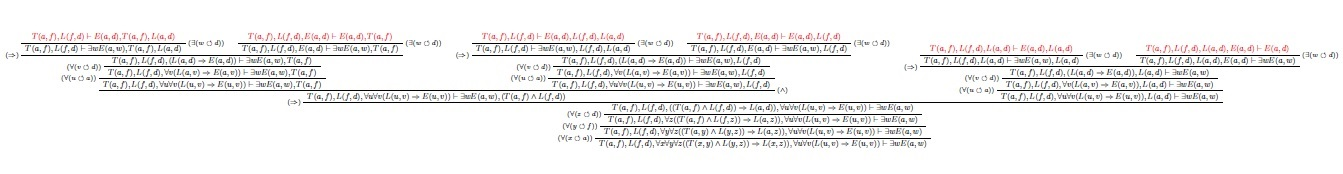
\includegraphics[width=24cm]{figures/RNFa}
    \end{turn}
    \caption[1 melleklet]{1. Példa bizonyítási fája}
    \label{fig-melleklet1}
\end{figure}

\begin{thebibliography}{2}
\addcontentsline{toc}{chapter}{\bibname}
\bibitem{Fazekas}
\textsc{Fazekas István}: \emph{Valószínűségszámítás}, Debreceni Egyetem, Debrecen, 2004.
\bibitem{Tomacs}
\textsc{Tómács Tibor}: \emph{A valószínűségszámítás alapjai}, Líceum Kiadó, Eger, 2005.
\bibitem{VartereszI1} \textsc{Várterész Magdolna}: \emph{Az informatika logika alapjai előadások}, 2006/07-es tanév 1.félév, \url{http://users.atw.hu/de-mi/index.php?r=file/download\&id=219},  Letöltve: 2019 március 12.-én
\end{thebibliography}
\chapter{Adatbázis ábra}
\centering
\includepdf{Hephaistos.pdf}

% Ide lehet szkennelt dokumentumot, dokumentumokat beszúrni
%\includepdf{}

\chapter*{Források}
\addcontentsline{toc}{chapter}{Források}
Az alábbi források kerültek felhasználásra a szakdolgozat elkészítése során:
\begin{itemize}
    \item \textsc{Fazekas István}: \emph{Valószínűségszámítás}, Debreceni Egyetem, Debrecen, 2004.
    \item \textsc{Tómács Tibor}: \emph{A valószínűségszámítás alapjai}, Líceum Kiadó, Eger, 2005.
    \item \textsc{Várterész Magdolna}: \emph{Az informatika logika alapjai előadások}, 2006/07-es tanév 1.félév, \url{http://users.atw.hu/de-mi/index.php?r=file/download\&id=219}, Letöltve: 2019 március 12.-én.
\end{itemize}

\end{document}

Antónia Beáta Varga <vargaa@kkszki.hu> ezt írta (időpont: 2025. ápr. 10., Cs, 9:03):
\documentclass[colorlinks]{thesis-kando}
\usepackage[T1]{fontenc}
\PassOptionsToPackage{defaults=hu-min}{magyar.ldf}
\usepackage[magyar]{babel}
\usepackage{graphicx,amsmath,amssymb,amsthm,hulipsum,bussproofs}
\usepackage{listings,xcolor,rotating,booktabs,fancyvrb}
\footnotestyle{rule=fourth}
\DeclareMathOperator{\tg}{tg}
\newtheorem{tetel}{Tétel}[chapter]
\usepackage[T1]{fontenc}
\PassOptionsToPackage{defaults=hu-min}{magyar.ldf}
\usepackage[magyar]{babel}
\usepackage{graphicx,amsmath,amssymb,amsthm,hulipsum,bussproofs}
\usepackage{listings,xcolor,rotating,booktabs,fancyvrb}
\footnotestyle{rule=fourth}
\newtheorem{lemma}[tetel]{Lemma}
\theoremstyle{definition}
\newtheorem{definicio}[tetel]{Definíció}
\newtheorem{feladat}[tetel]{Feladat}
\theoremstyle{remark}
\newtheorem{megjegyzes}[tetel]{Megjegyzés}
\newtheorem*{megoldas}{Megoldás}
\usepackage[utf8]{inputenc}
\usepackage[normalem]{ulem}
\usepackage{graphicx}
\usepackage{pdfpages}
\usepackage[linguistics]{forest}
\usepackage{stackengine,scalerel}

\usepackage[utf8]{inputenc} % ha még nincs
\usepackage{listings}
\usepackage{xcolor}

\lstset{
    inputencoding=utf8,
    extendedchars=true,
    literate={á}{{\'a}}1 {é}{{\'e}}1 {í}{{\'i}}1 {ó}{{\'o}}1 {ö}{{\"o}}1 {ő}{{\H{o}}}1
    {ú}{{\'u}}1 {ü}{{\"u}}1 {ű}{{\H{u}}}1
    {Á}{{\'A}}1 {É}{{\'E}}1 {Í}{{\'I}}1 {Ó}{{\'O}}1 {Ö}{{\"O}}1 {Ő}{{\H{O}}}1
    {Ú}{{\'U}}1 {Ü}{{\"U}}1 {Ű}{{\H{U}}}1,
    breaklines=true,
    basicstyle=\ttfamily\small,
    keywordstyle=\color{blue},
    commentstyle=\color{gray},
    stringstyle=\color{teal}
}


% Define JavaScript language for listings
\lstdefinelanguage{JavaScript}{
    keywords={break, case, catch, continue, debugger, default, delete, do, else, finally, for, function, if, in, instanceof, new, return, switch, this, throw, try, typeof, var, void, while, with, let, const, export, import, await, async},
    ndkeywords={class, export, boolean, throw, implements, import, this, new},
    sensitive=true,
    comment=[l]{//},
    morecomment=[s]{/*}{*/},
    morestring=[b]',
    morestring=[b]",
    alsoletter={-},
    alsodigit={:},
    morekeywords=[2]{=>, yield, async, await, constructor},
    keywordstyle=\color{blue}\bfseries,
    ndkeywordstyle=\color{green}\bfseries,
    identifierstyle=\color{black},
    commentstyle=\color{gray}\ttfamily,
    stringstyle=\color{red}\ttfamily,
}

% Customize listings appearance
\lstset{
    language=JavaScript,
    extendedchars=true,
    inputencoding=utf8,
    basicstyle=\ttfamily\small,
    numbers=left,
    numberstyle=\tiny\color{gray},
    stepnumber=1,
    numbersep=10pt,
    showstringspaces=false,
    breaklines=true,
    frame=single,
    captionpos=b,
    escapeinside={\%*}{*)},
}

% Fordított 'T' szimbólum definiálása
\def\tang{\ThisStyle{\abovebaseline[0pt]{\scalebox{-1}{$\SavedStyle\perp$}}}}

\begin{document}


\title{Project Hephaistos}

\author{Biliczki Bence\\Fodor Valentin Sándor\\Szegedi Dávid\\Szoftverfejlesztő és -tesztelő szak}

\supervisor{Kerényi Róbert Nándor\\oktató}
\city{Miskolc}
\date{2024}
\begin{figure}[h]
    \centering
    \label{fig:minta}
\end{figure}
\maketitle

\tableofcontents

\pagebreak

\section*{Bevezetés} \addcontentsline{toc}{section}{Bevezetés}

A Project Hephaistos egy innovatív, egyetemisták számára készült órarend-tervező alkalmazás, amely célja, hogy hatékonyan támogassa a hallgatókat az órák, tanórán kívüli tevékenységek és egyéb kötelezettségek rendszerezésében. Az alkalmazás C# nyelven készült, és egy gépészmérnökhallgató igényei alapján lett fejlesztve, különös figyelmet szentelve a funkcionalitásnak és a felhasználóbarát felületnek. Az intelligens ütemezési megoldások lehetővé teszik az egyéni preferenciák, az egyetemi órarend és az időbeli ütközések figyelembevételét.

\section{Használt Technológiák}
A Hephaistos projekt különböző, modern technológiákat alkalmaz a backend, frontend fejlesztéséhez, valamint az adatbázis kezeléséhez. A backend fejlesztés során erőteljes és skálázható megoldásokat biztosítanak, például Node.js használatával, amelyek lehetővé teszik a gyors, aszinkron feldolgozást és az API-k kialakítását. A backend kezelheti a felhasználói adatokat, autentikációt, valamint biztosítja az alkalmazás logikai rétegeit, és kezeli a kommunikációt az adatbázissal.

A frontend fejlesztésére a projekt React környezetben dolgozik, hogy dinamikus, interaktív felhasználói felületeket kínáljon, amelyek gyorsan reagálnak a felhasználói interakciókra. Ezek a könyvtárak lehetővé teszik a komponens-alapú struktúrák kialakítását, így a fejlesztés hatékonyabb és karbantarthatóbb lesz. A CSS preprocesorok és UI frameworkök (pl. Material-UI, Bootstrap) tovább javítják a felhasználói élményt és az alkalmazás megjelenését.

Az adatbázis-kezeléshez a projekt fejlesztése során MySQL relációs adatbázist használunk, amely lehetővé teszi az adatok hatékony tárolását és gyors lekérdezését. A backend és az adatbázis közötti kommunikációt közvetlen SQL lekérdezések segítségével végezzük, amelyek egyszerűsítik az adatok kezelését és lekérdezését az alkalmazás logikai rétegében. A projekt publikálása után az adatbázis az Azure felhőszolgáltatáson keresztül kerül elérhetővé, biztosítva a skálázhatóságot, megbízhatóságot és biztonságot a termelési környezetben. A Hephaistos projekt által használt technológiai stack elősegíti a rugalmas, skálázható és könnyen karbantartható alkalmazások fejlesztését, biztosítva a zökkenőmentes integrációt a backend, frontend és az adatbázis között.

\subsection{Backend}
A projekt backend fejlesztéséhez a .NET Core keretrendszert használjuk, amely egy nyílt forráskódú, platformfüggetlen fejlesztői környezet. A .NET Core lehetővé teszi a fejlesztők számára, hogy modern, felhőalapú alkalmazásokat építsenek, amelyek nagy teljesítményűek és könnyen skálázhatók. A keretrendszer előnye, hogy több operációs rendszeren is működik, beleértve a Windows, Linux és macOS platformokat, így rugalmas fejlesztési lehetőségeket kínál A .NET Core különösen jól támogatja a mikroszolgáltatás-alapú architektúrákat, így lehetőség van az alkalmazás kisebb, jól elkülöníthető szolgáltatásokra bontására. Ez nemcsak a karbantarthatóságot növeli, hanem biztosítja a magas rendelkezésre állást és skálázhatóságot is. Az integrációs lehetőségek, például a Microsoft Azure-val való zökkenőmentes együttműködés, lehetővé teszik a felhőszolgáltatások egyszerű használatát. A fejlesztés során az Entity Framework Core biztosítja az adatok kezelését, egyszerűsítve az adatbázisokkal való munkát, miközben a web API-k gyors létrehozására is lehetőséget ad, támogatva a RESTful szolgáltatásokat. Ezzel biztosítva van a könnyű adatkommunikáció a frontend és backend között.

\subsubsection{ASP.NET Core}
Az ASP.NET Core a .NET Core keretrendszer része, amelyet webalkalmazások és API-k fejlesztésére használnak. Az ASP.NET Core előnyei közé tartozik a magas teljesítmény, a platformfüggetlenség és a moduláris felépítés. Az ASP.NET Core támogatja a modern webfejlesztési szabványokat és eszközöket, mint például a dependency injection, a middleware-ek és a RESTful API-k.

Az ASP.NET Core alkalmazások könnyen telepíthetők és skálázhatók, így ideálisak a felhőalapú környezetekben történő futtatásra. Az ASP.NET Core lehetővé teszi a fejlesztők számára, hogy gyorsan és hatékonyan hozzanak létre biztonságos és megbízható webalkalmazásokat.

\subsection{Adatbázis}
Az adatok tárolására MySQL adatbázist használunk. A MySQL egy népszerű, nyílt forráskódú relációs adatbázis-kezelő rendszer, amely nagy teljesítményt és megbízhatóságot kínál. A PHPMyAdmin eszközt használjuk az adatbázis kezelésére, amely egy webalapú felületet biztosít az adatbázisok kezeléséhez.

\subsection{Frontend}
A React egy népszerű JavaScript-könyvtár, amelyet dinamikus és interaktív felhasználói felületek (UI) fejlesztésére használnak. A React lehetővé teszi a fejlesztők számára, hogy komponens-alapú módon építsenek fel alkalmazásokat, ahol minden komponens saját állapotot és viselkedést tartalmaz. A virtuális DOM használata gyorsabb renderelést biztosít, mivel csökkenti a tényleges DOM-műveletek számát. A React alkalmazásokat könnyen skálázhatjuk és karbantarthatjuk, és a könyvtár számos kiegészítő eszközt kínál, mint például Redux az állapotkezeléshez, vagy React Router a navigációhoz. Emellett a React lehetőséget ad mobilalkalmazások készítésére is React Native segítségével.



\subsubsection{React}
A React egy komponens-alapú JavaScript könyvtár, amelyet a Meta fejlesztett ki és 2013-ban adtak ki. A React fő célja a felhasználói felületek egyszerűbb és hatékonyabb fejlesztése. A React lehetővé teszi a fejlesztők számára, hogy újrafelhasználható komponenseket hozzanak létre, amelyek könnyen karbantarthatók és bővíthetők.

A React egyik legfontosabb jellemzője a virtuális DOM (Document Object Model), amely javítja az alkalmazás teljesítményét azáltal, hogy minimalizálja a valódi DOM manipulációkat. A React támogatja a JSX (JavaScript XML) szintaxist, amely lehetővé teszi a HTML-szerű kód írását a JavaScript-ben, növelve a kód olvashatóságát és karbantarthatóságát.

A React ökoszisztémája számos kiegészítő könyvtárat és eszközt tartalmaz, mint például a React Router a kliensoldali útvonalkezeléshez és a Redux az állapotkezeléshez. Ezek az eszközök segítenek a fejlesztőknek hatékonyabb és skálázhatóbb alkalmazásokat létrehozni.

\subsection{Fejlesztői Eszközök}
A fejlesztés során különböző eszközöket használunk a hatékonyság növelése és a hibakeresés megkönnyítése érdekében:
\begin{itemize}
    \item \textbf{Visual Studio Code (VSCode)}: Egy népszerű kódszerkesztő, amely számos bővítménnyel rendelkezik, például az \texttt{ESLint} és \texttt{Prettier} segítségével.
    \item \textbf{React Developer Tools}: Egy böngészőbővítmény, amely lehetővé teszi a React komponensek és állapotok ellenőrzését a böngészőben.
    \item \textbf{PHPMyAdmin}: Egy webalapú eszköz a MySQL adatbázisok kezelésére.
\end{itemize}

\section{Projekt Felépítése}
A Hephaistos projekt három fő komponensből áll: backend, frontend és adatbázis. Az alábbiakban bemutatjuk ezeknek a komponenseknek a felépítését és funkcióit.

\section{Órarend Generátor Funkció}
A Project Hephaistos backend tartalmaz egy órarend generátor funkciót, amely segíti a felhasználókat az optimális órarend összeállításában. Ez a funkció figyelembe veszi a felhasználó által teljesített tantárgyakat, a tantárgyak előfeltételeit, valamint az időbeli ütközéseket.

\subsection{TimetableGenerator Osztály}
A \texttt{TimetableGenerator} osztály felelős az órarend generálásáért. Az osztály a következő fő metódust tartalmazza:

\begin{itemize}
    \item \textbf{GenerateClosestTimetable}: Ez a metódus a megadott kreditszám alapján generál egy optimális órarendet. A metódus figyelembe veszi az elérhető tantárgyakat és az ütemezési konfliktusokat.
\end{itemize}

Az alábbi kód egy részletet mutat be a \texttt{GenerateClosestTimetable} metódusból:

\begin{lstlisting}[language=JavaScript]
public (IEnumerable<SubjectSchedule> Timetable, IEnumerable<Subject> OmittedSubjects) GenerateClosestTimetable(
    int creditValue,
    List<Subject> _availableSubjects,
    List<SubjectSchedule> _existingSchedules
) {
    var selectedSubjects = new List<Subject>();
    var omittedSubjects = new List<Subject>();
    var selectedSchedules = new List<SubjectSchedule>();
    int totalCredits = 0;

    foreach (var subject in _availableSubjects) {
        if (totalCredits + (subject.CreditValue ?? 0) > creditValue) {
            omittedSubjects.Add(subject);
            continue;
        }

        var subjectSchedules = _existingSchedules.Where(s => s.SubjectId == subject.Id).ToList();

        if (!subjectSchedules.Any(schedule => IsOverlapping(schedule, selectedSchedules))) {
            selectedSubjects.Add(subject);
            selectedSchedules.AddRange(subjectSchedules);
            totalCredits += subject.CreditValue ?? 0;
        } else {
            omittedSubjects.Add(subject);
        }
    }

    return (selectedSchedules, omittedSubjects);
}
\end{lstlisting}

\subsection{TimetableGeneratorController Végpont}
A \texttt{TimetableGeneratorController} egy API végpontot biztosít az órarend generálásához. A végpont a következőképpen működik:

\begin{itemize}
    \item \textbf{POST /api/timetablegenerator/generate}: Ez a végpont fogadja a felhasználó által megadott kreditszámot, és visszaadja az optimális órarendet, valamint azokat a tantárgyakat, amelyek kimaradtak az ütemezésből.
\end{itemize}

Az alábbi kód egy részletet mutat be a végpont implementációjából:

\begin{lstlisting}[language=JavaScript]
[HttpPost("generate")]
[Authorize]
public async Task<IActionResult> GenerateTimetable([FromBody] int creditValue, [FromHeader(Name = "Authorization")] string Authorization) {
    var userId = _jwtHelper.ExtractUserIdFromToken(Authorization);
    var availableSubjects = GetAvailableSubjects(userId.Value);
    var existingSchedules = _context.Subjectschedules
        .Where(schedule => availableSubjects.Any(subject => subject.Id == schedule.SubjectId))
        .ToList();

    var (timetable, omittedSubjects) = _timetableGenerator.GenerateClosestTimetable(creditValue, availableSubjects, existingSchedules);

    return Ok(new {
        Timetable = timetable.Select(schedule => new {
            SubjectName = schedule.Subject?.Name,
            DayOfWeek = schedule.DayOfWeek,
            StartTime = schedule.StartTime,
            EndTime = schedule.EndTime
        }),
        OmittedSubjects = omittedSubjects.Select(subject => new {
            SubjectName = subject.Name
        })
    });
}
\end{lstlisting}

\subsection{Felhasználói Élmény}
A funkció biztosítja, hogy a felhasználók egy könnyen értelmezhető órarendet kapjanak, amely tartalmazza az órák nevét, időpontját és napját. Az ütemezésből kimaradt tantárgyak külön listában jelennek meg, hogy a felhasználók tisztában legyenek azokkal a tantárgyakkal, amelyeket nem sikerült beilleszteni az órarendbe.

\chapter{Relációs adatkezelő rendszerek}

\section{Relációs adatbázis}

Relációs adatbázisnak nevezzük azokat az adatbázisokat, amelyek a relációs adatmodell elvein alapulnak. Ezekben az adatok táblázatos formában, ún. relációkban (táblákban) vannak tárolva, ahol a sorok egyedi rekordokat, az oszlopok pedig mezőket (attribútumokat) jelentenek. A relációs adatbázis több ilyen táblát tartalmaz, amelyeket egymással kapcsolatokon (kulcsokon) keresztül lehet összekötni. Az ilyen adatbázisokat relációs adatbázis-kezelő rendszerek (pl. MySQL, PostgreSQL, SQL Server) segítségével lehet létrehozni, módosítani és kezelni. Az adatok lekérdezésére és módosítására jellemzően az SQL nyelvet használjuk. A relációs adatbázisok erőssége a strukturált adattárolás, a konzisztencia és az adatintegritás biztosítása.

\subsection{A relációs adatbáziskezelő rendszerek}

A relációs adatbáziskezelő rendszerek (RDBMS, azaz Relational Database Management System) olyan szoftverek, amelyek az adatokat táblák formájában kezelik. Minden tábla oszlopokból és sorokból áll, ahol az oszlopok különböző attribútumokat jelölnek, míg a sorok egyedi rekordokat reprezentálnak. Az RDBMS-ekben a táblák között relációk, azaz kapcsolatok hozhatók létre, így biztosítva az adatok egymáshoz kapcsolódó kezelését.

Az RDBMS-ek egyik legfontosabb jellemzője a strukturált lekérdezőnyelv, azaz az SQL (Structured Query Language), amely lehetővé teszi az adatok lekérdezését, módosítását és kezelését. Az adatokat kulcsok segítségével kapcsoljuk össze, mint például az elsődleges kulcs (primary key) és az idegen kulcs (foreign key). Az adatok normalizálásával csökkenthetők az ismétlődések, és fenntartható az adatintegritás. A relációs adatbáziskezelő rendszerek széles körben elterjedtek különböző üzleti és technológiai területeken, mivel lehetővé teszik az adatok hatékony tárolását és kezelését, valamint a nagy mennyiségű adat gyors lekérdezését.
\pagebreak
\subsection{MySQL és MariaDB, valamint PHPMyAdmin}

A MySQL és a MariaDB két népszerű, nyílt forráskódú relációs adatbáziskezelő rendszer. Mindkettő hasonló struktúrát és működési elveket követ, mivel a MariaDB a MySQL-ből származik. A MySQL-t eredetileg a Sun Microsystems fejlesztette ki, majd a Sun felvásárlása után az Oracle tulajdonába került. A MariaDB-t a MySQL eredeti fejlesztői hozták létre az Oracle irányításától való függetlenség megőrzése érdekében, és azóta külön fejlesztési irányt követ.

Mindkét rendszer könnyen kezelhető, nagy teljesítményt és skálázhatóságot kínál, így gyakran használják webalkalmazások és más dinamikus rendszerek adatbázisaként. A MySQL és a MariaDB támogatják a különféle táblastruktúrákat (például InnoDB és MyISAM), a tranzakciókezelést, valamint a különféle biztonsági mechanizmusokat, mint például a felhasználói jogosultságok finomhangolása.

A PHPMyAdmin egy népszerű, nyílt forráskódú webes eszköz, amelyet kifejezetten MySQL és MariaDB adatbázisok kezelésére fejlesztettek ki. Lehetővé teszi a felhasználók számára, hogy grafikus felületen keresztül, SQL parancsok írása nélkül menedzseljék az adatbázisokat. Ezzel az eszközzel könnyen létrehozhatók és módosíthatók táblák, kezelhetők a felhasználói jogosultságok, és futtathatók különböző SQL lekérdezések.

A PHPMyAdmin előnye, hogy böngésző alapú, így bármilyen eszközről könnyen elérhető, nem szükséges hozzá parancssori ismeret. A felhasználók könnyen átláthatják az adatbázis struktúráját, létrehozhatnak exportálási és importálási műveleteket, valamint automatikusan generált diagramok segítségével áttekinthetik a táblák közötti kapcsolatokat. Ezen kívül a PHPMyAdmin lehetőséget biztosít biztonsági mentések készítésére, így a felhasználók megőrizhetik és helyreállíthatják az adatokat.

\begin{figure}[ht!]
    \centering
    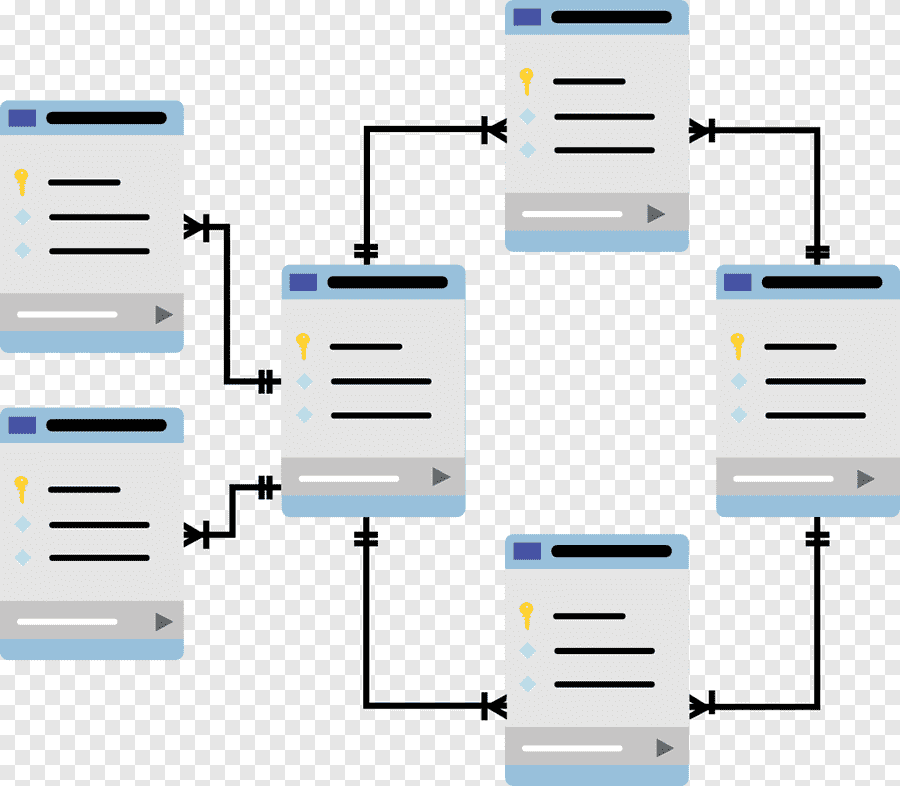
\includegraphics[width=9cm]{figures/rdb.png}
    \caption[dotNET]{Relációs adatbázis}
\end{figure}
\pagebreak

\chapter{React Fejlesztői Környezet}

\section{Bevezetés}
A React egy népszerű JavaScript-könyvtár, amelyet a felhasználói felületek egyszerűbb fejlesztésére használnak. Ezt a Meta fejlesztette, és 2013-ban adták ki. Azóta széles körben alkalmazzák a webes fejlesztésben, különösen az egyoldalas alkalmazások (SPA) készítéséhez. Ez a szakdolgozat a React fejlesztői környezetek felépítését, a szükséges eszközöket és a hatékony fejlesztéshez szükséges alapelveket vizsgálja.

\section{React Fejlesztői Környezet}
Ebben a fejezetben bemutatjuk a React fejlesztői környezet telepítését, a szükséges eszközöket, valamint a React alapjait, hogy a fejlesztés hatékony és eredményes legyen.

\subsection{React Telepítése és Projektindítás}
A React telepítéséhez először szükségünk van a Node.js és npm (Node Package Manager) telepítésére, amelyek segítségével kezelhetjük a JavaScript könyvtárakat és függőségeket. Miután a Node.js és az npm telepítve van, létrehozhatunk egy új React projektet az \texttt{create-react-app} eszközzel.

Az alábbi parancsokkal létrehozható egy új React projekt:
\begin{lstlisting}[language=bash]
npx create-react-app my-app
cd my-app
npm start
\end{lstlisting}

\pagebreak

A \texttt{create-react-app} gyorsan felállít egy alap React projektstruktúrát, amely a következő fájlokat tartalmazza:
\begin{itemize}
    \item \texttt{src/} mappa: tartalmazza a forráskódot, beleértve a komponenseket és az alkalmazás logikáját.
    \item \texttt{public/} mappa: statikus fájlokat, például képeket és index.html-t tartalmazza.
    \item \texttt{node\_modules/}: az összes szükséges függőséget tartalmazza.
\end{itemize}

\subsection{Fejlesztői Eszközök}
A React fejlesztéséhez számos fejlesztői eszköz áll rendelkezésünkre, amelyek növelhetik a termelékenységet és a hibakeresés hatékonyságát.


\subsubsection{React Developer Tools}
A React Developer Tools egy hivatalos böngészőbővítmény, amely lehetővé teszi a React alapú webalkalmazások mélyreható vizsgálatát és hibakeresését közvetlenül a böngésző fejlesztői eszközein belül. A bővítmény segítségével a fejlesztők átlátható módon megtekinthetik az alkalmazás teljes komponensfáját, beleértve a komponensek közötti hierarchiát és kapcsolatokat. Különösen hasznos funkciója, hogy lehetővé teszi az egyes komponensekhez tartozó props és state értékek valós idejű megfigyelését, illetve ezek változásainak nyomon követését a felhasználói interakciók során. A modern React fejlesztés során gyakran használt Hook-ok – mint például a useState, useEffect, vagy useContext – szintén jól követhetők a bővítményen keresztül, így a fejlesztők részletes információt kaphatnak az alkalmazás belső állapotairól. Ezen kívül a React Developer Tools egy beépített profilozó eszközt is tartalmaz, amely lehetővé teszi a komponensrenderelések teljesítményének elemzését, megmutatva, hogy mely komponensek renderelődnek újra, milyen gyakorisággal, és mennyi idő alatt. Mindezek együttesen nagyban hozzájárulnak a hatékonyabb hibakereséshez, az optimalizáláshoz, és az alkalmazás működésének jobb megértéséhez, ezáltal elengedhetetlenné téve a bővítményt minden komolyabb React fejlesztési projekt során.

\section{React Alapjai}
A React egy összetevő-alapú megközelítést alkalmaz, amelyben az alkalmazás kisebb, újrafelhasználható komponensekből épül fel. Ez a moduláris felépítés segít a kód karbantartásában és a fejlesztés gyorsításában.

\subsection{Komponensek és JSX}
A React komponensek JavaScript függvények vagy osztályok, amelyek HTML-szerű kódot, úgynevezett JSX-et használnak. A JSX lehetővé teszi, hogy a JavaScript kódban HTML elemeket írjunk, ami növeli a kód olvashatóságát.

\section*{Microsoft Azure Elérhetőség}
\addcontentsline{toc}{section}{Microsoft Azure Elérhetőség}
A Project Hephaistos alkalmazásunkat a Microsoft Azure felhőszolgáltatás segítségével publikáltuk, amely lehetővé teszi a skálázható és megbízható működést. Az Azure biztosítja az alkalmazás számára a szükséges infrastruktúrát, beleértve a webalkalmazás hosztolását, az adatbázis-kezelést és a biztonságos hozzáférést.

Az alkalmazás elérhető az alábbi linken:
\url{https://hephaistos-backend-c6c5ewhraedvgzex.germanywestcentral-01.azurewebsites.net/index.html}

\subsection*{Azure Szolgáltatások Használata}
A projekt során az alábbi Azure szolgáltatásokat használtuk:
\begin{itemize}
    \item \textbf{Azure App Service}: Az alkalmazás hosztolására és futtatására használtuk. Ez egy teljesen menedzselt platform, amely lehetővé teszi a gyors telepítést és a folyamatos integrációt.
    \item \textbf{Azure SQL Database}: Az alkalmazás adatainak tárolására és kezelésére szolgál. Ez egy skálázható, biztonságos és megbízható relációs adatbázis-kezelő rendszer.
    \item \textbf{Azure Monitor}: Az alkalmazás teljesítményének és állapotának nyomon követésére használtuk. Ez segít az esetleges problémák gyors azonosításában és megoldásában.
    \item \textbf{Azure Active Directory (AAD)}: A felhasználók hitelesítésére és az alkalmazás biztonságának növelésére használtuk.
\end{itemize}

\subsection*{Előnyök}
A Microsoft Azure használata számos előnyt biztosít a projekt számára:
\begin{itemize}
    \item \textbf{Skálázhatóság}: Az alkalmazás könnyen skálázható a felhasználói igények növekedésével.
    \item \textbf{Megerősített Biztonság}: Az Azure beépített biztonsági funkciói, például a titkosítás és a hozzáférés-szabályozás, garantálják az adatok védelmét.
    \item \textbf{Globális Elérhetőség}: Az Azure globális adatközpont-hálózata lehetővé teszi az alkalmazás gyors és megbízható elérését a világ bármely pontjáról.
    \item \textbf{Költséghatékonyság}: Az Azure rugalmas árazási modellje lehetővé teszi, hogy csak a ténylegesen használt erőforrásokért fizessünk.
\end{itemize}

A Microsoft Azure segítségével biztosítjuk, hogy a Project Hephaistos alkalmazás \href{https://projecthephaistos.azurewebsites.net/index.html} megbízhatóan és hatékonyan szolgálja ki a felhasználók igényeit.

\addcontentsline{toc}{section}{Elérhetőség}
\pagebreak

\begin{lstlisting}[language=JavaScript]
import React from 'react';


function Welcome(props) {
    return <h1>Hello, {props.name}</h1>;
}

export default Welcome;
\end{lstlisting}

\subsection{Állapotkezelés a React-ben}
A React komponensek állapotkezelése alapvető fontosságú a dinamikus, interaktív felhasználói felületek létrehozásához. Az állapot (state) lehetővé teszi, hogy a komponens megőrizze az aktuális adatállapotát, és reagáljon a felhasználói interakciókra, például kattintásokra vagy űrlapváltozásokra. Az useState Hook segítségével egyszerűen létrehozhatunk és módosíthatunk állapotokat, amelyek hatására a komponens újrarenderelődik, és a felület frissül. Egyszerűbb alkalmazásoknál elegendő a helyi állapotkezelés, míg komplexebb esetekben érdemes globális megoldásokat is alkalmazni, például a Context API-t vagy Reduxot. Az állapotkezelés tehát kulcsfontosságú eszköz a React-komponensek viselkedésének irányításához és a felhasználói élmény kialakításához.

\subsubsection{useState Hook}
A \texttt{useState} egy hook, amely lehetővé teszi az állapotkezelést a funkcionális komponensekben. Az alábbi példa egy egyszerű számlálót mutat be, amely a \texttt{useState} használatával kezeli az állapotot:

\begin{lstlisting}[language=JavaScript]
import React, { useState } from 'react';

function Counter() {
    const [count, setCount] = useState(0);

    return (
        <div>
            <p>You clicked {count} times</p>
            <button onClick={() => setCount(count + 1)}>
                Click me
            </button>
        </div>
    );
}

export default Counter;
\end{lstlisting}

\subsection{Props}
A React komponensek közötti kommunikációt az úgynevezett \texttt{props} (properties) segítségével valósítják meg. A \texttt{props} adatokat továbbítanak az egyik komponensből a másikba.

\begin{lstlisting}[language = JavaScript]
function Greeting(props) {
    return <h1>Hello, {props.name}</h1>;
}

function App() {
    return <Greeting name="React Developer" />;
}

export default App;
\end{lstlisting}

\subsection{Komponensek Típusai}
A React komponensek két fő típusa:
\begin{itemize}
    \item \textbf{Funkcionális komponensek}: egyszerű JavaScript függvények, amelyek a \texttt{props}-ot paraméterként veszik át és JSX-et adnak vissza.
    \item \textbf{Osztály alapú komponensek}: osztályok, amelyek bonyolultabb állapotkezelést és életciklus-módszereket tesznek lehetővé.
\end{itemize}

\pagebreak


\section{Jelszó Módosítása Funkció}
A React frontend alkalmazás tartalmaz egy jelszó módosítási funkciót, amely lehetővé teszi a felhasználók számára, hogy biztonságosan megváltoztassák a jelszavukat. Ez a funkció a következő komponensekből áll:

\subsection{ChangePasswordForm Komponens}
A \texttt{ChangePasswordForm} egy React komponens, amely biztosítja a jelszó módosításához szükséges űrlapot. Az űrlap tartalmaz mezőket a régi jelszó, az új jelszó és az új jelszó megerősítésének megadásához. Az alábbi kód egy részletet mutat be a komponensből:

\begin{lstlisting}[language=JavaScript]
    import React, { useState } from 'react';

    function ChangePasswordForm() {
        const [oldPassword, setOldPassword] = useState('');
        const [newPassword, setNewPassword] = useState('');
        const [confirmPassword, setConfirmPassword] = useState('');

        const handleChangePassword = () => {
            if (newPassword !== confirmPassword) {
                alert('Az új jelszavak nem egyeznek!');
                return;
            }
            // Jelszó módosítási logika
        };

        return (
        <form>
        <input type="password" placeholder="Régi jelszó" onChange={(e) => setOldPassword(e.target.value)} />
        <input type="password" placeholder="Új jelszó" onChange={(e) => setNewPassword(e.target.value)} />
        <input type="password" placeholder="Új jelszó megerősítése" onChange={(e) => setConfirmPassword(e.target.value)} />
        <button type="button" onClick={handleChangePassword}>Jelszó módosítása</button>
        </form>
        );
    }
\end{lstlisting}

\subsection{Backend Integráció}
A jelszó módosítási funkció a backend API-val kommunikál, hogy ellenőrizze a régi jelszót és frissítse az új jelszót az adatbázisban. Az API végpontja a következő:

\begin{lstlisting}[language=JavaScript]
POST https://localhost:5001/change-password
Headers: {
    Authorization: Bearer <token>
}
Body: {
    "oldPassword": "current_password",
    "newPassword": "new_password"
}
\end{lstlisting}

\subsection{Felhasználói Élmény}
A funkció biztosítja, hogy a felhasználók értesítést kapjanak a sikeres vagy sikertelen jelszó módosításról. A hibák, például a nem egyező jelszavak vagy a helytelen régi jelszó, azonnal megjelennek az űrlapon.

\end{document}


\section{Összefoglalás}
A React fejlesztői környezet és eszköztár megismerése elengedhetetlen a hatékony fejlesztési folyamat érdekében. A fenti fejezetekben bemutattuk a telepítést, az állapotkezelést, a komponenseket és azok életciklusát, valamint néhány fontos React fejlesztői eszközt.

\newpage
\Huge\begin{center}
    \textbf{Köszönetnyilvánítás}
\end{center}\normalsize
Szeretnék köszönetet mondani mindazoknak, akik segítették a vizsgaremekem létrejöttét, külön megköszönve
\newline\newline

\begin{figure}[ht!]
    \centering
    \begin{turn}{90}
        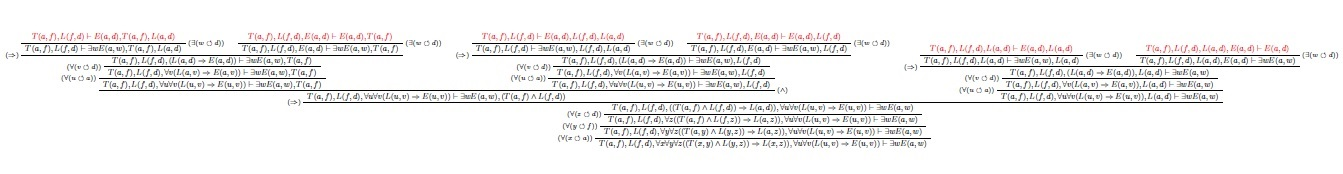
\includegraphics[width=24cm]{figures/RNFa}
    \end{turn}
    \caption[1 melleklet]{1. Példa bizonyítási fája}
    \label{fig-melleklet1}
\end{figure}

\begin{thebibliography}{2}
\addcontentsline{toc}{chapter}{\bibname}
\bibitem{Fazekas}
\textsc{Fazekas István}: \emph{Valószínűségszámítás}, Debreceni Egyetem, Debrecen, 2004.
\bibitem{Tomacs}
\textsc{Tómács Tibor}: \emph{A valószínűségszámítás alapjai}, Líceum Kiadó, Eger, 2005.
\bibitem{VartereszI1} \textsc{Várterész Magdolna}: \emph{Az informatika logika alapjai előadások}, 2006/07-es tanév 1.félév, \url{http://users.atw.hu/de-mi/index.php?r=file/download\&id=219},  Letöltve: 2019 március 12.-én
\end{thebibliography}
\chapter{Adatbázis ábra}
\centering
\includepdf{Hephaistos.pdf}

% Ide lehet szkennelt dokumentumot, dokumentumokat beszúrni
%\includepdf{}

\chapter*{Források}
\addcontentsline{toc}{chapter}{Források}
Az alábbi források kerültek felhasználásra a szakdolgozat elkészítése során:
\begin{itemize}
    \item \textsc{Fazekas István}: \emph{Valószínűségszámítás}, Debreceni Egyetem, Debrecen, 2004.
    \item \textsc{Tómács Tibor}: \emph{A valószínűségszámítás alapjai}, Líceum Kiadó, Eger, 2005.
    \item \textsc{Várterész Magdolna}: \emph{Az informatika logika alapjai előadások}, 2006/07-es tanév 1.félév, \url{http://users.atw.hu/de-mi/index.php?r=file/download\&id=219}, Letöltve: 2019 március 12.-én.
\end{itemize}

\end{document}